% Chapter 3
\chapter{Derivation of Functional Requirements from Use Cases} % Main chapter title

\label{Chapter3} % For referencing the chapter elsewhere, use \ref{Chapter1} 

%----------------------------------------------------------------------------------------
This chapter gives a list of the required use cases of the secure phone. A list of functional requirements has then been created based upon the needs of the use cases. 
\begin{figure}
	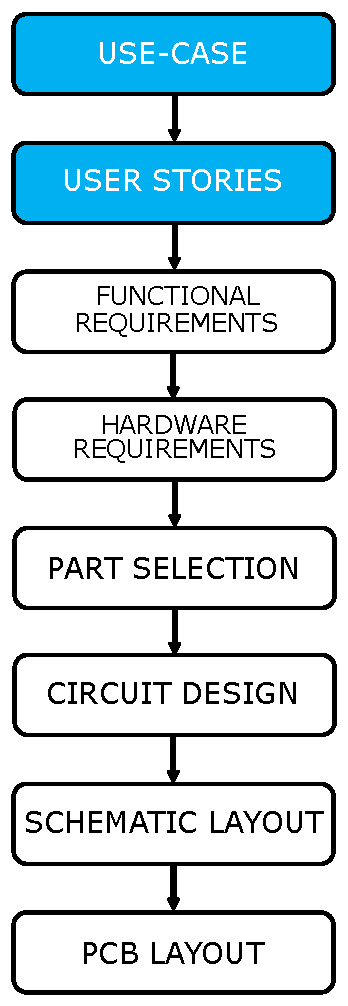
\includegraphics[height=0.5\linewidth]{Figures/usecases.pdf}\centering
	\caption{Design Process}
	\label{fig:methodology}
\end{figure}

\section{Use Cases}

	For the project a number of use cases were identified which needed to be satisfied. The following list describes the use cases and the functional requirements for which how they would be satisfied;

\subsection{Voice telephony}
	This basic phone requirement would require the use of both a speaker, a microphone and a SIM card slot as well as software to be able to communicate between the user and the receiver. The requirement would also needed at least one modem, ideally two, to allow true dual-sim, dual-network operation. In terms of software, this would require the telephony software, which has already been developed.\\

        \subsubsection{User Story}
        ''Joe picks up his MEGAphone out of his bag, presses the power button to wake it up, then uses the touch screen to select the dialer application, searches for his friend Bob in the contact list using the DPAD to quickly scan through the list, but can't find it, so manually enters his number using the dial pad on the touch screen, and presses the call button and holds the MEGAphone to his ear.  The MEGAphone establishes the call, and Bob and Joe talk with each for some time before hanging up.  Soon after, realising he forgot to tell Joe something, Bob calls Joe back, causing Joe's MEGAphone to ring.  Joe answers the call using the touch screen, puts the call on speaker-phone while writing down the information from Bob, before thanking him and hanging up.''

        \subsubsection{Functional Requirements}
        \begin{itemize}
        \item MEGAphone is a portable phone-like device.
        \item MEGAphone can operate using battery power.
        \item MEGAphone has a power button, that when pressed wakes the device.
        \item MEGAphone has a display.
        \item MEGAphone has a touch-digitiser on its display.
        \item MEGAphone has an application launcher.
        \item MEGAphone has dialer software.
        \item MEGAphone has a DPAD (4-way thumb joystick).
        \item MEGAphone has a cellular modem.
        \item MEGAphone can place cellular voice calls.
        \item MEGAphone has a microphone.
        \item MEGAphone has an earpiece.
        \item MEGAphone can route audio from the microphone to cellular modem.
        \item MEGAphone can route audio from the cellular modem to the earpiece.
        \item MEGAphone can ring when it is called.
        \item MEGAphone has a speaker-phone mode.
        \end{itemize}

\subsection{Text messaging}
	Again this use case would require at least one modem and at least one SIM card slot. This would also work with the telephony software already developed.\\

	\subsubsection{User Story}
	''Lisa takes out her MEGAphone from her bag, presses the power button to wake it up, then uses the touch screen to select the dialer application. Lisa then uses the DPAD to search for her friend in the contact list, uses the touch screen to select the friend, then presses the button to enter the text messaging screen. Lisa then uses the on-screen keyboard to enter in her text using the touch screen and presses the send button. A little while later Lisa receives a text back from the person she first sent a text to.''

        \subsubsection{Functional Requirements}
        \begin{itemize}
        \item MEGAphone is a portable phone-like device.
        \item MEGAphone can operate using battery power.
        \item MEGAphone has a power button, that when pressed wakes the device.
        \item MEGAphone has a display.
        \item MEGAphone has a touch-digitiser on its display.
        \item MEGAphone has an application launcher.
        \item MEGAphone has dialer software.
        \item MEGAphone has a DPAD (4-way thumb joystick).
        \item MEGAphone has a cellular modem.
	\item MEGAphone dialer software includes an on-screen keyboard.
	\item MEGAphone can send and recieve text messages.
        \end{itemize}

\subsection{Highly secure communication (One-Time Pad Encryption)}
	This would primarily need a NOR Flash, to be able to work with a device with a different pad and NOR Flash.\\

	\subsubsection{User Story}
	''Paul pulls out his MEGAphone and decides to send a confidential message to his friend. ''

        \subsubsection{Functional Requirements}
        \begin{itemize}
        \item MEGAphone is a portable phone-like device.
        \item MEGAphone can operate using battery power.
        \item MEGAphone has a power button, that when pressed wakes the device.
        \item MEGAphone has a display.
        \item MEGAphone has a touch-digitiser on its display.
        \item MEGAphone has an application launcher.
        \item MEGAphone has dialer software.
        \item MEGAphone has a DPAD (4-way thumb joystick).
        \item MEGAphone has a cellular modem.
	\item MEGAphone dialer software includes an on-screen keyboard.
	\item MEGAphone can send and recieve text messages.
	\item MEGAphone has a NOR Flash
	\item MEGAphone utilises OTP
        \end{itemize}

\subsection{Playing 8-bit videogames}
	This would require the traditional game controller aspects; DPAD, push buttons, etc. This would also require the device to have pre-loaded games, and that the buttons on the device correctly map to the required targets in the game.\\

	\subsubsection{User Story}
	''Jill takes out her MEGAphone and wakes it up using the power button. Using the touch screen, Jill loads the game that she wants to play and waits for the game to load. Once loaded, Jill uses the DPAD and A and B buttons to navigate her way through the game. During the game, she uses the thumbwheel at the bottom of the phone to turn down the sound.''

        \subsubsection{Functional Requirements}
        \begin{itemize}
        \item MEGAphone is a portable phone-like device.
        \item MEGAphone can operate using battery power.
        \item MEGAphone has a power button, that when pressed wakes the device.
        \item MEGAphone has a display.
        \item MEGAphone has a touch-digitiser on its display.
        \item MEGAphone has an application launcher.
        \item MEGAphone has a DPAD (4-way thumb joystick).
        \item MEGAphone has multiple buttons for varied purposes.
	\item MEGAphone has a thumbwheel so that the volume can be modified.
        \end{itemize}

\subsection{Listening to music}
	This would require the use of speakers, and software to be able to play the music. This would also require certain software to be able to pick, choose and play music.\\

	\subsubsection{User Story}
	''Jeff wakes his MEGAphone uses the power button and uses the touch screen to navigate to the music software on the phone. Jeff uses the DPAD to easily scroll through the music available on the inserted MicroSD card, and selects the song.''

        \subsubsection{Functional Requirements}
        \begin{itemize}
        \item MEGAphone is a portable phone-like device.
        \item MEGAphone can operate using battery power.
        \item MEGAphone has a power button, that when pressed wakes the device.
        \item MEGAphone has a display.
        \item MEGAphone has a touch-digitiser on its display.
        \item MEGAphone has an application launcher.
        \item MEGAphone has music software.
        \item MEGAphone has a DPAD (4-way thumb joystick).
	\item MEGAphone has a thumbwheel so that the volume can be modified.
	\item MEGAphone has two speakers.
	\item MEGAphone has MicroSD storage capability.
        \end{itemize}

\subsection{Store data}
	This would require at least one MicroSD slot, to be able to store data and use the data on the device. This would also require software to be able to interact with the data and transfer it.\\

	\subsubsection{User Story}
	''Harry takes out his MEGAphone and wakes it up using the power button. Wanting to play an audio file, Harry inserts a 32Gb MicroSD card into the MicroSD card slot, and uses the application launcher to find the content.''

        \subsubsection{Functional Requirements}
        \begin{itemize}
        \item MEGAphone is a portable phone-like device.
        \item MEGAphone can operate using battery power.
        \item MEGAphone has a power button, that when pressed wakes the device.
        \item MEGAphone has a display.
        \item MEGAphone has a touch-digitiser on its display.
        \item MEGAphone has an application launcher.
        \item MEGAphone has a DPAD (4-way thumb joystick).
	\item MEGAphone has MicroSD storage capability.
        \end{itemize}
%----------------------------------------------------------------------------------------

\section{Functional Requirements}
	
	The following list displays the functional requirements of the phone, based upon the use case requirements.\\
	\begin{itemize}
        \item MEGAphone is a portable phone-like device.
        \item MEGAphone can operate using battery power.
        \item MEGAphone has a power button, that when pressed wakes the device.
        \item MEGAphone has a display.
        \item MEGAphone has a touch-digitiser on its display.
        \item MEGAphone has an application launcher.
        \item MEGAphone has dialer software.
        \item MEGAphone has a DPAD (4-way thumb joystick).
        \item MEGAphone has a cellular modem.
        \item MEGAphone can place cellular voice calls.
        \item MEGAphone has a microphone.
        \item MEGAphone has an earpiece.
        \item MEGAphone can route audio from the microphone to cellular modem.
        \item MEGAphone can route audio from the cellular modem to the earpiece.
        \item MEGAphone can ring when it is called.
        \item MEGAphone has a speaker-phone mode.
	\item MEGAphone has MicroSD storage capability.
	\item MEGAphone has a thumbwheel so that the volume can be modified.
	\item MEGAphone has two speakers.
	\item MEGAphone dialer software includes an on-screen keyboard.
	\item MEGAphone can send and recieve text messages.
	\item MEGAphone has a NOR Flash
	\item MEGAphone utilises OTP
	\end{itemize}
